\documentclass[12pt, a4paper, titlepage]{article}

% VARIABLES
% Change these to suit your essay.
\def\thetitle{SDP Group Report - Milestone 1}
\def\theauthor{Group 4}

% FONTS
\usepackage{fontspec} 
\usepackage{xunicode}
\usepackage{xltxtra}
\defaultfontfeatures{Mapping=tex-text}
\setromanfont[Ligatures={Common},
	BoldFont={Adobe Garamond Pro Bold},
	ItalicFont={Adobe Garamond Pro Italic}]{Adobe Garamond Pro}
\setmonofont[Scale=0.8]{Monaco} 

% DOCUMENT LAYOUT
\usepackage{geometry} 
% Change this if you have specific margins to use.
\geometry{a4paper, left=0.8in, right=0.8in}

% HEADERS
\usepackage{fancyhdr}
\pagestyle{fancyplain}
\rhead{\textsc{\theauthor}}
\lhead{\textsc{SDP Group Report - Milestone 1}}
\setlength{\headheight}{14.5pt}

% HEADINGS
\usepackage{sectsty} 
\usepackage[normalem]{ulem} 
\sectionfont{\rmfamily\bfseries\upshape\Large}
\subsectionfont{\rmfamily\bfseries\upshape\normalsize} 
\subsubsectionfont{\rmfamily\mdseries\upshape\normalsize} 

\usepackage{titlesec}
\titleformat{\section}{\large\bfseries\raggedright}{}{0em}{\thesection\hspace{1em}}[\titlerule]

% SYMBOLS & MATHS
\usepackage{amsmath}
\usepackage{marvosym}
\usepackage{url}

% SOURCE CODE
\usepackage{minted}

% TODOs
\usepackage{todonotes}

% GRAPHICS
\usepackage{titlepic}
\usepackage{graphicx}

% PDF SETUP
\usepackage[dvipdfm,bookmarks,colorlinks,breaklinks,pdftitle={\thetitle},pdfauthor={\theauthor}]{hyperref}  
\hypersetup{linkcolor=black,citecolor=black,filecolor=black,urlcolor=blue} 

% TITLE PAGE
\setlength{\headsep}{5mm}

\title{\small{SDP Group Report - Milestone 1} \\ \huge Group 4 -- Castle Crashers}
\author{Andrew Johnstone \and Callum Stott \and Christopher Brown \and Daniel Wren \and Emil Georgiev \and Katherine Findlay \and Magdelena Konkiewicz \and Sittikorn Assavanives \and Steven Skelton \and William Bradshaw}
\date{\today}
\titlepic{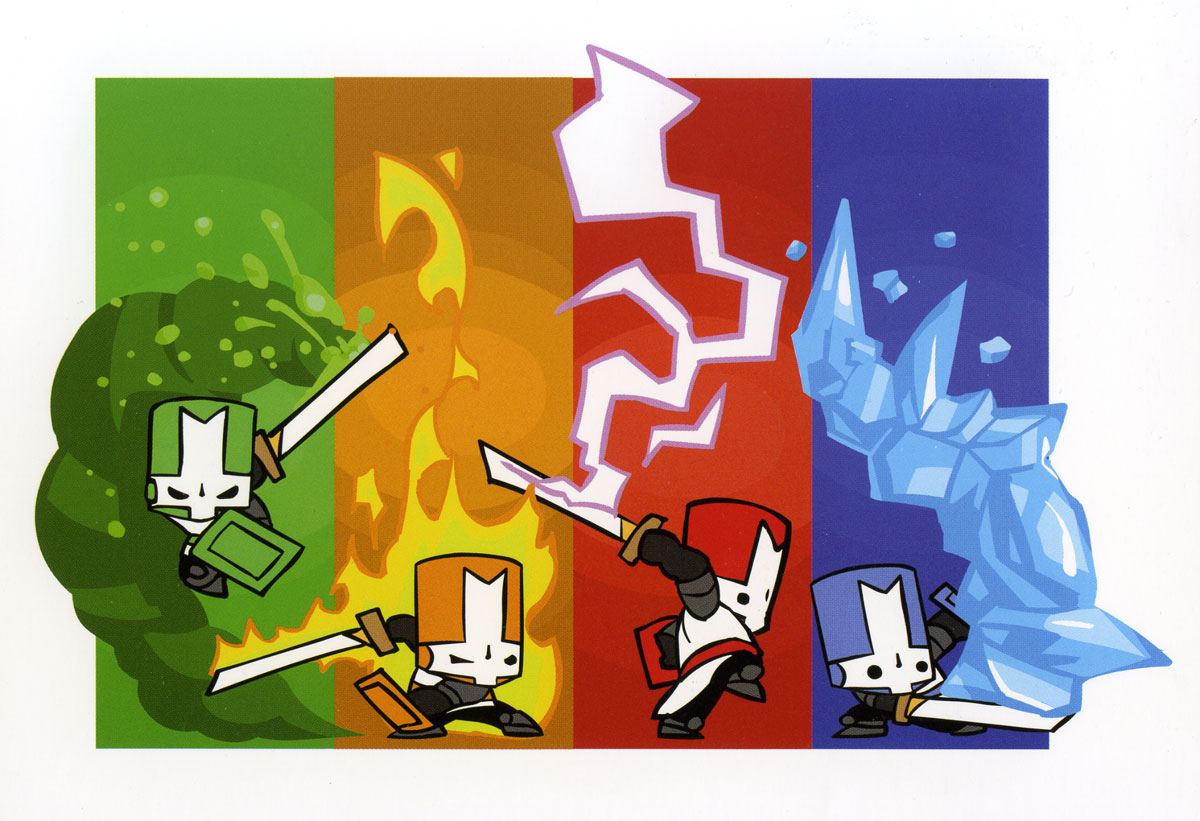
\includegraphics[width=0.8\textwidth]{images/team-logo.jpg}\\[1cm]}

\begin{document}
\maketitle

\section{Introduction}

Over the first two weeks of the System Design Project (SDP) our team has made
fantastic progress with our project to build football playing robots. We have
surpassed the requirements for the first milestone and are working hard to reach
the second one soon.

\section{Programming \& Vision}

The programming and vision section of our team has three main subsections:
robot control and communication, vision, and strategy. For the first milestone
it was essential that we could control the robot remotely. This priority meant
that we assigned two programmers (Callum, Chris) to work on robot movement and
communication to ensure that it was ready for the first milestone. Another
programmer (Steven) was tasked with creating the vision system for the project.
Since the vision wasn't essential for milestone one, but is critical for
milestone two, more programmers will be assigned to work on it. The strategy
element of the programming has been started by another programmer (Andrew) who
migrated to programming after working on the construction for the first
week.

\subsection{Control \& Communication}

The first task for the control and communication sub-project was to decide which
software we should use for the firmware replacement on the NXT device and on
the computer to control the robot. We found a piece of software called
leJOS\cite{lejos} which seemed to be a perfect candidate due to the fact that
it was written in Java, had an API for both the robot and the computer and, was
a stable and mature project.

As we now had a small code base - that was growing as we were trying out new
things - we decided that our next task would be to set up version control
for our team. Everyone in the programming team was keen to use a distributed
version control system as we knew that it would suit our branch-heavy work flow.
We decided to use Git\cite{git-scm} for this task as some of the group were
familiar with it already.

After this was completed we moved on to programming ``real'' code for the
robot instead of the demos we had been running up until now. We set up a basic
protocol for the robot and the computer to communicate with. Our first major
problem was that some of the motor control commands block the running thread.
This meant that commands were being stopped in the command streams and the other
unrelated commands cannot be run. To fix this we implemented a command loop
pattern running in a different thread to handle the commands. This threw up
some initial concurrency issues but these were soon fixed and we could continue
working with the engineering team to implement the new features. Magdelena sent
us a patch that allowed the robot to react to the newly fitted sensors and move
away from any dangers or obstacles.

Towards the end of the two weeks we began to document our code and set up build
systems (Ant\cite{ant}) to allow for other team members who had not been working
on the code to get up to speed and start contributing. As of now, we have a
simple interface to control the robot and are ready to start integrating all of
our distinct systems together.

\subsection{Vision}

We researched possible software libraries to perform the image analysis needed
for this task. While researching we came across the OpenCV library\cite{opencv}.
A key advantage to OpenCV was that it is written in C and is therefore fast
at processing images compared to other languages. Initially OpenCV wasn't
installed on the DICE systems so a separate laptop was used. Once the software
was installed it was apparent that there were errors in the installation. While
OpenCV did work, only the Python wrapper could be used. From here we decided to
rewrite our program using the OpenCV Python wrapper bindings instead.

Our algorithm captures an image from the live feed. Image noise is reduced by
downscaling to a smaller resolution and then back to the original resolution,
resulting in the image being slightly blurred. We then convert the input image
from RGB to the HSV colour space to allow for the easier isolation of colours.
We create a binary image from a certain colour in the image. This binary
image appears white where the required colour is found in the image and black
everywhere else. The white area is located in the image and once the object has
been found the coordinates are returned and a bounding box is drawn around it on
the live image.

\subsection{Strategy}

The initial goal of the strategy sub-project was to make a start towards the
completion of our second milestone: moving towards the ball. To facilitate this
research was done into path-finding algorithms such as depth-first searching.

After much consideration A* searching was chosen as it provided both an accurate
and high performance method for calculating routes. A simple simulation was
run of the algorithm that calculated a path between an object and a point on a
simple field, which was successful. This simple implementation will require some
modification before it usable for our purposes. Preliminary work was also made
to determine a good heuristic for this algorithm, but this is an area that will
require further testing.

\section{Engineering \& Construction}

In order to build a successful robot we decided to focus on speed,
maneuverability, and kicker strength. We also decided to cover as much area as
possible so that we would be better at blocking goals. The design of our robot
was influenced heavily by Lego castle walls, these pieces cover a large area
while being sturdy and light.

\subsection{Movement}

Our initial design involved two wheels at the front connected to individual
motors and using one small wheel at the back to handle turning. The result
of this was a robot that could move quickly while at the same time turning
smoothly. We tried using four normal wheels with gears to speed up the movement.
By connecting two motors to the front wheels and using gears alongside the
Lego Technic beams to connect the back wheels. This design gives decent speed
but the problem with this design is the robot cannot turn sideways smoothly as
the wheels jump off the pitch while turning. Our final design uses tank tracks
along the sides of the robot. This is by far the fastest moving and turning of
all other designs. However, there is a slight problem as the robot slips while
moving, because the tracks have insufficient friction.

\subsection{Kicker}

The kicker, unlike much of our design, went through a number of different
prototypes. We toyed with various ideas, all powered by an NXT motor, using
different structures and gearing. Some of our designs include examples such as
a kicker made up of long blocks stacked up (to present a large face) but this
proved too heavy. Another prototype was made from more castle walls but again we
thought we could push the design further and when we implemented the spinner we
made up our new kicker out of basic reinforced bars so as to follow our mantra
of ``light and sturdy''. We are satisfied with the power our kicker currently
offers but cannot help but feel that through some testing and more prototypes we
can improve it through either using another motor or a gearing system.

\subsection{Spinner}

A spinner of sorts was implemented. It works by using RCX motors to power
a pulley system. The pulleys then power a large wheel that is used to spin
additional wheels built into our kicker. The spinner applies back spin to the
ball so that the robot can control it to a certain degree by keeping it close
enough to get maximum force out of each kick. This system in no way removes the
ball from play, it merely rolls the ball toward our robot to keep it close.

\subsection{Sensors}

We have decided to use two touch sensors at the front of the robot, placed on
the left and right side of the kicker, and one ultrasonic sensor at the back.
We also have tested the robot with sensors which were placed much higher (about
10 cm from the ground), which would still detect the walls of the pitch but
possibly not the robot's opponent. However, we have decided that it is important
to recognize both walls and the opponent, and agreed to place the sensors on
the lower level. For similar reasons we have implemented one ultrasonic sensor
at the back placing it about 5 cm from the ground. Figures~\ref{fig:frontview}
and~\ref{fig:backview} show the actual placement of the sensors in our robot. We
also decided not to have any sensors at the sides of the robot, as it is using
tank tracks which limits the movement to backwards and forwards directions.

\section{Future Plans}

Before the next deadline we will attempt to integrate the separate systems we
have into a larger single system. The robot will be controlled autonomously
based on inputs from the camera. In order to test this we need to have made a
start on a simulator for our strategy. For the next milestone we aim to have a
working simulator and the robot will be able to make decisions about what to do
based on the world state.

On the robot side we are going to be interweaving two rubber bands through each
tank track. This gives our robot more speed (by reducing “slippage”) and
better traction, furthermore it increases the precision of our turning on the
spot, offering precise 90, 180 and 360 degree turns.

\newpage

\setcounter{section}{5}
\begin{thebibliography}{9}

\bibitem{lejos}
	leJOS,
	\url{http://lejos.sourceforge.net}

\bibitem{git-scm}
	Git Source Control Management,
	\url{http://git-scm.com}

\bibitem{ant}
	Apache Ant,
	\url{http://ant.apache.org/}

\bibitem{opencv}
	OpenCV,
	\url{http://opencv.willowgarage.com/wiki/}

\end{thebibliography}

\appendix
\section{Photographs}

\begin{figure}[h]
\begin{minipage}[b]{0.5\linewidth}
\centering
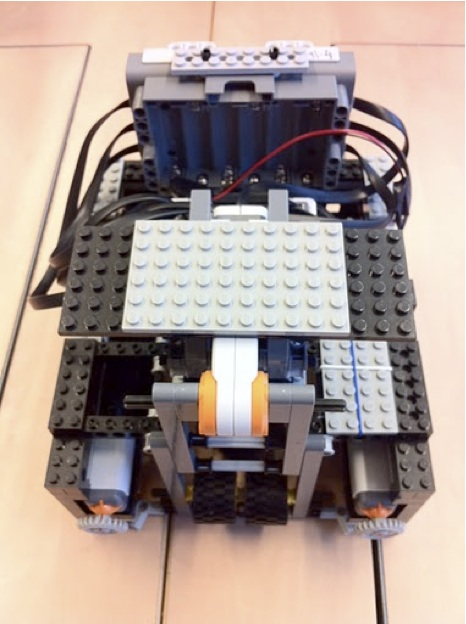
\includegraphics[scale=0.8]{images/robot/topview.jpg}
\caption{Top View}
\label{fig:topview}
\end{minipage}
\hspace{0.5cm}
\begin{minipage}[b]{0.5\linewidth}
\centering
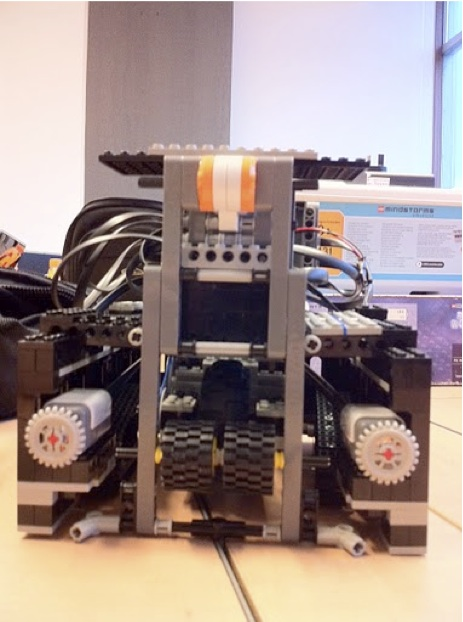
\includegraphics[scale=0.8]{images/robot/frontview.jpg}
\caption{Front View}
\label{fig:frontview}
\end{minipage}
\end{figure}

\begin{figure}[ht]
\begin{minipage}[b]{0.5\linewidth}
\centering
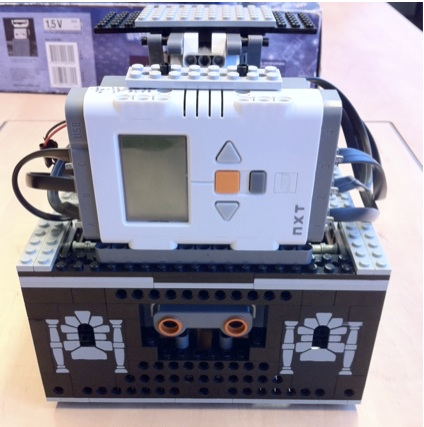
\includegraphics[scale=0.8]{images/robot/backview.jpg}
\caption{Back View}
\label{fig:backview}
\end{minipage}
\hspace{0.5cm}
\begin{minipage}[b]{0.5\linewidth}
\centering
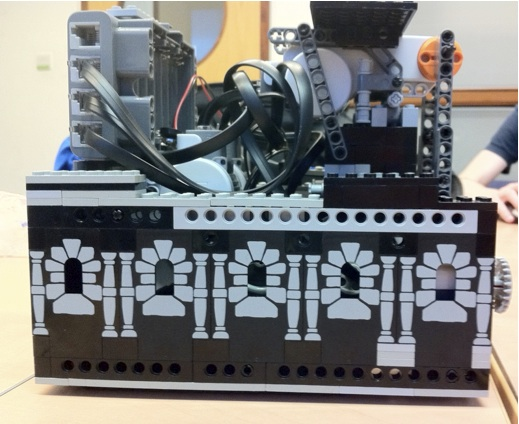
\includegraphics[scale=0.8]{images/robot/sideview.jpg}
\caption{Side View}
\label{fig:sideview}
\end{minipage}
\end{figure}

\begin{figure}[ht]
\begin{minipage}[b]{0.5\linewidth}
\centering
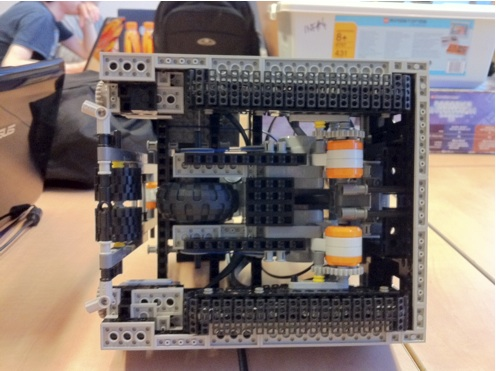
\includegraphics[scale=0.8]{images/robot/bottomview.jpg}
\caption{Tank Tracks}
\label{fig:tanktracks}
\end{minipage}
\hspace{0.5cm}
\begin{minipage}[b]{0.5\linewidth}
\centering
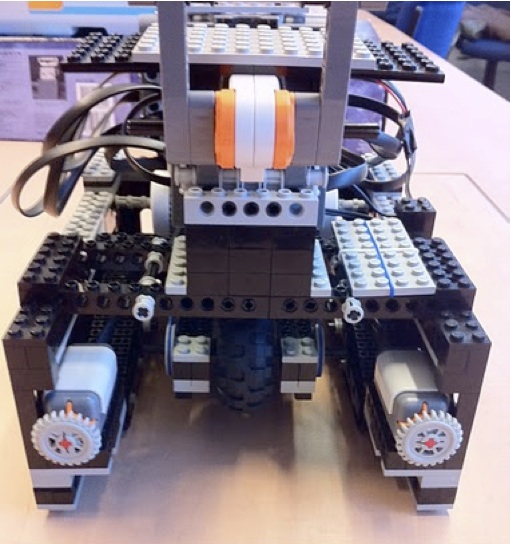
\includegraphics[scale=0.8]{images/robot/driver.jpg}
\caption{Driver}
\label{fig:driver}
\end{minipage}
\end{figure}

\begin{figure}[ht]
\begin{centering}
\begin{minipage}[b]{0.3\linewidth}
\centering
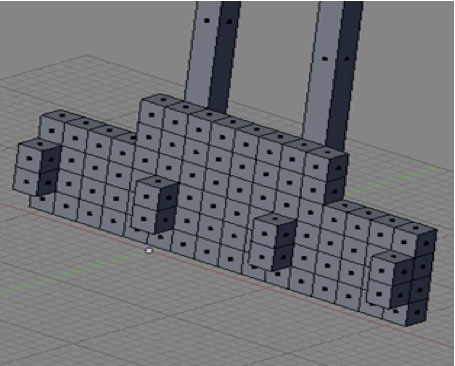
\includegraphics[scale=0.5]{images/robot/firstkicker.jpg}
\caption{First Kicker}
\label{fig:firstkicker}
\end{minipage}
\hspace{0.3cm}
\begin{minipage}[b]{0.3\linewidth}
\centering
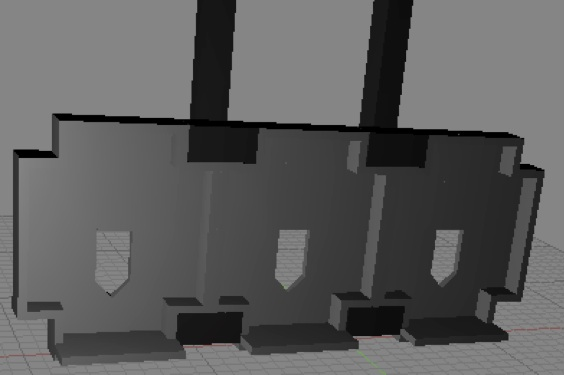
\includegraphics[scale=0.5]{images/robot/secondkicker.jpg}
\caption{Second Kicker}
\label{fig:secondkicker}
\end{minipage}
\hspace{0.3cm}
\begin{minipage}[b]{0.3\linewidth}
\centering
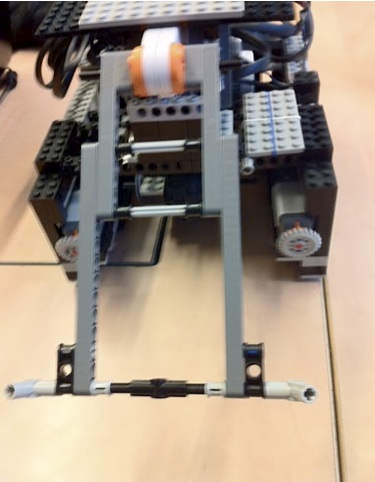
\includegraphics[scale=0.5]{images/robot/thirdkicker.jpg}
\caption{Third Kicker}
\label{fig:thirdkicker}
\end{minipage}
\end{centering}
\end{figure}

\begin{figure}[ht]
\centering
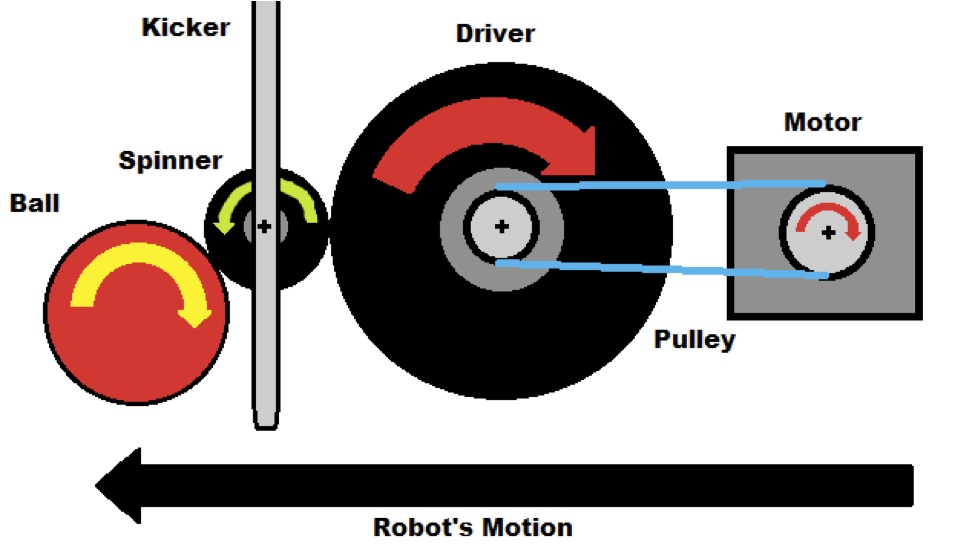
\includegraphics[scale=0.8]{images/robot/spinner.jpg}
\caption{Spinner Diagram}
\label{fig:spinner}
\end{figure}

\end{document}
